% REMEMBER: You must not plagiarise anything in your report. Be extremely careful.

\documentclass{l4proj}

    
%
% put any additional packages here
%

\begin{document}

%==============================================================================
%% METADATA
\title{Level 4 Project Report Template}
\author{John H. Williamson}
\date{September 14, 2018}

\maketitle

%==============================================================================
%% ABSTRACT
\begin{abstract}
    Every abstract follows a similar pattern. Motivate; set aims; describe work; explain results.
    \vskip 0.5em
    ``XYZ is bad. This project investigated ABC to determine if it was better. 
    ABC used XXX and YYY to implement ZZZ. This is particularly interesting as XXX and YYY have
    never been used together. It was found that  
    ABC was 20\% better than XYZ, though it caused rabies in half of subjects.''
\end{abstract}

%==============================================================================

% EDUCATION REUSE CONSENT FORM
% If you consent to your project being shown to future students for educational purposes
% then insert your name and the date below to  sign the education use form that appears in the front of the document. 
% You must explicitly give consent if you wish to do so.
% If you sign, your project may be included in the Hall of Fame if it scores particularly highly.
%
% Please note that you are under no obligation to sign 
% this declaration, but doing so would help future students.
%
%\def\consentname {My Name} % your full name
%\def\consentdate {20 March 2018} % the date you agree
%
\educationalconsent


%==============================================================================
\tableofcontents

%==============================================================================
%% Notes on formatting
%==============================================================================
% The first page, abstract and table of contents are numbered using Roman numerals and are not
% included in the page count. 
%
% From now on pages are numbered
% using Arabic numerals. Therefore, immediately after the first call to \chapter we need the call
% \pagenumbering{arabic} and this should be called once only in the document. 
%
% Do not alter the bibliography style.
%
% The first Chapter should then be on page 1. You are allowed 40 pages for a 40 credit project and 30 pages for a 
% 20 credit report. This includes everything numbered in Arabic numerals (excluding front matter) up
% to but excluding the appendices and bibliography.
%
% You must not alter text size (it is currently 10pt) or alter margins or spacing.
%
%
%==================================================================================================================================
%
% IMPORTANT
% The chapter headings here are **suggestions**. You don't have to follow this model if
% it doesn't fit your project. Every project should have an introduction and conclusion,
% however. 
%
%==================================================================================================================================
\chapter{Introduction}

% reset page numbering. Don't remove this!
\pagenumbering{arabic} 


Why should the reader care about what are you doing and what are you actually doing?
\section{Guidance}

\textbf{Motivate} 
Activity trackers are very popular nowadays. These apps leverage various motivators, such as social feeds, points for activity, and reminders. However, most of these apps do not leverage collaborative motivators. I wanted to investigate whether or not users would feel more motivated to exercise if it wasn't just about working towards a personal goal, but towards a shared goal with a team of friends/strangers. The goal of my RPG themed activity tracker, 'Stat Buff' was to gamify progress as ingame character development (leading to greater attack damage), and workouts as attacks towards your teams enemy. This rewards users for making progress in their performance, as well as for making small daily efforts. The teams enemy resets in a week if it has not been defeated, which creates an urgency to exercise in order to to reach the next enemy.
\section{Writing guidance}
\subsection{Who is the reader?}

This is the key question for any writing. Your reader:

\begin{itemize}
    \item
    is a trained computer scientist: \emph{don't explain basics}.
    \item
    has limited time: \emph{keep on topic}.
    \item
    has no idea why anyone would want to do this: \emph{motivate clearly}
    \item
    might not know \emph{anything} about your project in particular:
    \emph{explain your project}.
    \item
    but might know precise details and check them: \emph{be precise and
    strive for accuracy.}
    \item
    doesn't know or care about you: \emph{personal discussions are
    irrelevant}.
\end{itemize}

Remember, you will be marked by your supervisor and one or more members
of staff. You might also have your project read by a prize-awarding
committee or possibly a future employer. Bear that in mind.

\subsection{References and style guides}
There are many style guides on good English writing. You don't need to
read these, but they will improve how you write.

\begin{itemize}
    \item
    \emph{How to write a great research paper} \cite{Pey17} (\textbf{recommended}, even though you aren't writing a research paper)
    \item
    \emph{How to Write with Style} \cite{Von80}. Short and easy to read. Available online.
    \item
    \emph{Style: The Basics of Clarity and Grace} \cite{Wil09} A very popular modern English style guide.
    \item
    \emph{The Elements of Style} \cite{StrWhi07} Outdated, and American, but a classic.
    \item
    \emph{The Sense of Style} \cite{Pin15} Excellent, though quite in-depth.
\end{itemize}

\subsubsection{Citation styles}

%\item If you are referring to a reference as a noun, then cite it as: ``\citet{Orw68} discusses the role of language in political thought.''
%\item If you are referring implicitly to references, use: ``There are many good books on writing \citep{Orw68, Wil09, Pin15}.''

There is a complete guide on good citation practice by Peter Coxhead available here: \url{http://www.cs.bham.ac.uk/~pxc/refs/index.html}. 
If you are unsure about how to cite online sources, please see this guide: \url{https://student.unsw.edu.au/how-do-i-cite-electronic-sources}.

\subsection{Plagiarism warning}

\begin{highlight_title}{WARNING}
    
    If you include material from other sources without full and correct attribution, you are commiting plagiarism. The penalties for plagiarism are severe.
    Quote any included text and cite it correctly. Cite all images, figures, etc. clearly in the caption of the figure.
\end{highlight_title}


%==================================================================================================================================
\chapter{Background}
The most similar research I could find on collaborative activity trackers was a paper on an app named 'Pass the Ball' cite{}. This app was very simple: a team has one ball, and the person with that ball could score points for the team by exercising, and pass it to others. This very simple idea lead to many feeling responsibility to exercise when they had the ball. It also lead to lots of issues: users hogging the ball, stealing the ball for a point penalty, etc. There were also issues for users with irregular schedules. This study made me understand the importance of accountability and structure, but also the possible friction that this can cause if not implemented well. I also looked into a case study on 'Spy Feet' cite{} which was a pedometer that let the user progress in a story through walking. The researchers were I did some research into the effectiveness of activity trackers. Although this was singleplayer and story based, it was reassuring to see that gamified abstractions motivated users to exercise more. I also did some research into the state of activity trackers as a whole. 'Behavior Change Techniques in Top-Ranked Mobile Apps for Physical Activity' cite{} talked about the lack of behavioural change techniques employed in top apps, aswell as the two primary categories: educational and motivational. This made me consider which route I should take (I leaned more towards motivational, with educational aspects). 'Apps of Steel: Are Exercise Apps Providing Consumers With Realistic Expectations?' came to the same conclusion as the earlier paper: apps don't use enough behavioural change techniques. I kept this in mind, but still kept my focus on collaborative aspects. I also read 'Personalizing Mobile Fitness Apps Using Reinforcement Learning', as I was interested in if it was possible to increase the effectiveness of the collaborative techniques through machine learning. This was out of scope to implement due to a lack of experience and time. I read 'A Tale of Two Perspectives: A Conceptual Framework of User Expectations and Experiences of Instructional Fitness Apps' in order to understand what users prioritize in activity trackers. The app found that content was most important for 47.2%, technical implementation and utilities 39.7%, and psychological features were the most important for 13.2% of users. Because of this, I decided that I should pay attention to content and technical details even if they aren't what is being studied, as this will make the app more attractive and usable for participants. Finally, I did some research into behaviour change by looking at 'Integrated Theory of Health Behavior Change'. } I didn't have the time to implement most techniques, but it gave me a good understanding of how social support can be leveraged to drive behavioural change.

I analyzed existing exercise apps, and existing RPG games in order to better understand the two categories I am combining. I analyzed Stronglifts 5x5 and Jefit, two popular exercise apps. Both had inbuilt social features, and online forums to keep people motivated. They had some complicated exercise features like planning workouts that were out of scope for me. I found that Jefit had competitions, but no team based exercising. This clearly shows that there is space in the market for my app. I also analyzed existing RPG/fantasy mobile games. I found that the multiplayer games often had collaborative aspects: for instance, Clash of Clans has clans, were users need to give each other troops in order to optimally defend themselves. In many classic RPG games such as World of Warcraft, users often take specific roles, such as healer, tank, and damage dealer, who all have to work together to defeat harder and harder enemies. It was clear that collaboration was very important for existing multiplayer RPG/fantasy games. From this, I gathered that I should follow the RPG/fantasy model for collaboration, as it has been perfected over years.
\section{Guidance}
\begin{itemize}    
    \item
      Don't give a laundry list of references.
    \item
      Tie everything you say to your problem.
    \item
      Present an argument.
    \item Think critically; weigh up the contribution of the background and put it in context.    
    \item
      \textbf{Don't write a tutorial}; provide background and cite
      references for further information.
\end{itemize}

%==================================================================================================================================
\chapter{Analysis/Requirements}
Exercise is hard to do consistently, leading to high inactivity. Social and group based exercise (such as exercising with a friend or joining a class) are good solution for making people feel accountable, and forcing a schedule. Even then, exercise would still be for your own good, and not for some common goal. A collaborative activity tracker would try to remove the buy in of group based exercise (course cost, fixed schedule) and would make the user feel as though they were contributing to a collective success and not just an individual one.
\section{Guidance}
Make it clear how you derived the constrained form of your problem via a clear and logical process. 

%==================================================================================================================================
\chapter{Design}
I wanted this app to calculate your team's contribution based on your effort and your strength. Rewarding effort should hopefully motivate users to workout regularly and push themselves, even when progress plateaus. Progress is rarely a straight line: it often has bumps, but through perseverance, you progress more than you regress. This also motivates users with lots of experience, as they can often feel demotivated by the waning progress, and the amount of time and effort it can take to accomplish something a beginner can achieve in a fraction of the time. I also reward strength, as I want the app to provide users with long term motivation. I don't want users to simply exercise for the sake of exercise, but also for the long-term improvements in strength. Rewarding progression is also important as it disincentivizes overtraining. If I only reward effort, the optimal strategy would be to exercise as much as possible, even if you feel pain and your progression stops and regresses. By rewarding strength improvements, I reward the user for training moderately and resting adequately, as these are integral for long term progress. I gamify strength as attack damage, and effort as the number of attacks you deliver towards your team's enemy. The product of the two is the total damage that you deal towards your team's enemy. This total damage is the gamified abstraction of your contribution to your team.

After deciding that what I would need to measure, I had to decide how to quantify it. Effort is pretty difficult to measure. I could compare the user's per exercise performance relative to the last time. This would have a lot of confounding factors: personal differences and skill level let some add more weight with less effort. There would also be the problem of missing data (what is the effort on your first workout, or when you use new exercises?). This would also require users to input the number of repetitions and lifted weight for all their sets for all their exercises. Finally, this wouldn't reward users for putting in effort even on a bad day or during a plateau. I consulted sport science literature, and found a popular metric for estimating effort called RPE (Rate of Perceived Exertion). RPE is a scale from 1-10, where 1 is almost no effort, 5 is moderate effort, and 10 is maximal effort. RPE has the downside of not being objective, as we are relying on a person's subjective perception of their effort. Research by Monica et al. found that "The odds of underestimating RPE for an exerciser were 3.67 times greater than a non-exerciser" \cite{RPE_estimations}. This could be offset by reducing the RPE that beginner's estimate, but this was out of scope for this project. I am not particularly worried about intentional dishonesty with regards to RPE, as users can lie about the number of sets they complete, how much they can lift, how often they train, etc. I decided to use RIR (repetitions in reserve) as it seemed easier to understand than RPE. This article \cite{rir} made a good case for measuring total training stress through average RIR and total sets . I couldn't find any specific equations that combined the two, so I created this in order to calculate the total number of attacks that a user deals: 

\begin{lstlisting}[language=python, caption={Total of number of granted attacks based on average RIR and total sets}]
total_attacks = min(0, (10 - average_rir) * total_sets)
\end{lstlisting}

This reduces the number of dealt attacks as you have a higher RIR, and as you do less sets. This allows users to do more sets if they don't like pushing themselves too hard, and vice versa. 

The second value that I had to quantify strength, or attack damage. I wanted strength to be calculated relative to the person performing it. For example, it is harder for an average 50kg person to lift a certain weight, than for the average 80kg person. By taking this into account, I made the app more inclusive, and allowed everyone to contribute based on how strong they are relative to others like them, and not everyone else. Relative strength is simply a percentile that is calculated based on the demographic of the person, the exercise they performed, and the weight and repetitions that they used. There are sites which perform this calculation, which I will go into more detail in the implementation section. I was still left with the challenge of converting per-exercise percentiles into a single strength value. Initially, I used a simple naive implementation, where I took the mean of all exercises, and used that as the final strength value. I realized that this was problematic 


\chapter{Implementation}
\subsection{Server/Database}
The server is built with a technology called Postgraphile GraphQL. GraphQL is a query language similar to REST, except GraphQL requests require you to pass JSON keys which you require the values for. This is what a simple GraphQL request might look like: 

\begin{lstlisting}[language=python, caption={An example GraphQL query fetching information about user "orek" and their messages }, label=lst:callahan]
  query{
    user(username: "orek"){
      groupname
      createdAt
      updatedAt
      chatMessagesByUsername{
        nodes{
          textContent
          createdAt
        }
      }
    }
  }
\end{lstlisting}

\begin{lstlisting}[language=python, caption={Server response to the above query}]
  {
    "data": {
      "user": {
        "groupname": "Team Public",
        "createdAt": "2021-02-18T20:30:55.784356+02:00",
        "updatedAt": "2021-02-18T20:30:55.784356+02:00",
        "chatMessagesByUsername": {
          "nodes": [
            {
              "textContent": "Good day today, right?",
              "createdAt": "2021-02-18T20:30:55.784356+02:00"
            }
          ]
        }
      }
    }
  }
\end{lstlisting}
This query format has many benefits: a client would never overfetch or underfetch. In a standard REST setup, the /user endpoint might return user metadata and /messages might return a users messages. This would mean that the client would have to send two requests, which would be slower for both the client and the server. One solution might be setting up a single endpoint, /user\_messages, which returns both user metadata and user messages. This would have the downside of overfetching: whenever we needed just the user metadata, the server would still have to do extra work to fetch messages, leading to a slower query. GraphQL only requires one request to get exactly the data that you need, no more, and no less. The data also comes in the exact shape that you request it in, which makes mapping the data on the client easy. 

This sounds good in practice, but GraphQL can often perform poorly. This was brought to my attention by this video where Awad talks about the Waterfall problem. This is characterized by GraphQL resolvers sending needlessly many database queries to fetch data. In order to implement nested resolvers (such as fetching the child books from the parent library) you need to define a function which returns children based on parent values (such as fetching all books whose foreign key matches the parent's ID). In this case, we make one query to fetch library information, and another one to fetch all books. But what if we fetch all pages of each book? This would lead to potentially thousands of database queries, as each book would call it's child resolver function fetching it's pages. This could be executed in a single SQL query by using joins.

Luckily there is a library for this. Instead of issuing an SQL query for every single child in the query, Postgraphile acts as a middleware, converting GraphQL requests into a single SQL query. This has huge performance benefits over the afformentioned manual implementation, as only one SQL query is required, and SQL's optimization can be harnessed better (such as through indexes). Another huge benefit of Postgraphile is that it analyzes your databases, and generates your entire query API from analyzing attributes and relations in your database. A lot of my time usually goes in to writing, debugging and maintaining basic CRUD server logic. When the database becomes complicated, changing the structure and relationships of tables can require a lot of work to change on the server. Postgraphile removes all this effort. Postgraphile does require some configuration, as we usually want to grant and limit data access depending on user, and internal logic beyond simply reading and writing data.


\subsection{Security}
I am used to implementing security logic in the middleware, and not the database, so this was hard for to understand and implement. 

Removing read/write queries from the GraphQL API for specific fields and tables is very simple:

\begin{lstlisting}[language=SQL, caption={This comment tells Postgraphile to omit password fields} ]
comment on column "user".password is E'@omit';
\end{lstlisting}

The difficult part was implementing per user security. When a user signs up, their username is stored along with their salted and hashed password. They receive a JWT token containing their username and a expiry date, which is symmetrically encrypted by a secret key (to prevent anyone from issuing access tokens). 
\begin{figure}[bp!]
    \centering
    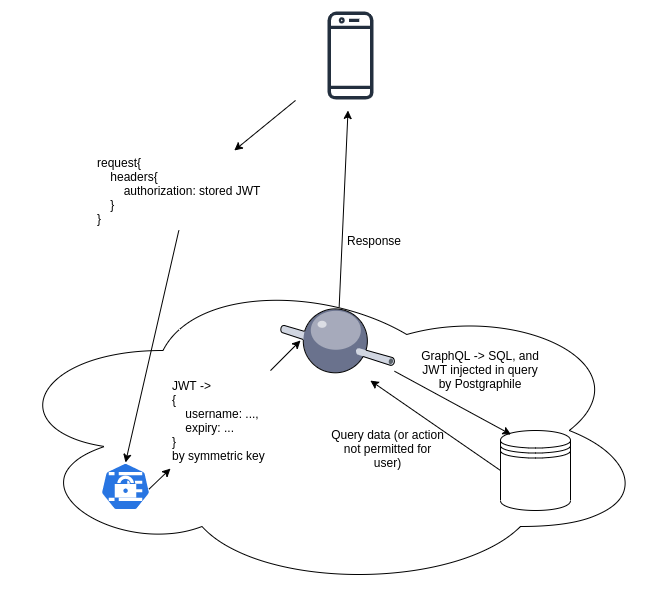
\includegraphics[width=1.0\linewidth]{authentication.png}    

    \caption{
  Once the user has stored the JWT token, this is how authentication works
    }
\end{figure}

Now that the database can authenticate users, it still needs to check whether or not a particular user has rights to perform an operation. This is implemented through row level security policies. Row level security policies only allow operations if the affected row(s) evaluate to true for the supplied boolean expression.


\begin{lstlisting}[language=SQL, caption={Row level security policies for accessing chat messages}, ]
CREATE POLICY chat_message_update ON "chat_message" FOR update to query_sender USING (username = (select username from active_user()));
CREATE POLICY chat_message_delete ON "chat_message" FOR delete to query_sender USING (username = (select username from active_user()));
CREATE POLICY chat_message_create ON "chat_message" FOR insert to query_sender with check (username = (select username from active_user()) and groupName = (select groupName from active_user()));
CREATE POLICY chat_message_select ON "chat_message" FOR select to query_sender using (groupName = (select groupName from active_user()));
\end{lstlisting}

The following code only allows a user to delete or update their own messages. Insert's are only allowed if the user also belongs to the group the message is sent to. Finally, any user in the group is allowed to read their group's messages. This combined with the earlier authentication protects unpermitted data access on the database itself. Although verbose, this creates consistent rules that can be written once and enforced everywhere, and prevents bugs that cause data leaks (for instance, sending all user data instead of filtering just the authenticated user's data, as this wouldn't be permitted by the RLS policies).

Finally, I will discuss password management. When a user creates an account by sending an encrypted POST request, I hash and salt the password and store the username in plaintext.

\begin{lstlisting}[language=SQL, caption={Hashing and salting done with pgcrypto}]
insert into "user"(username, password) values (username, crypt(password, gen_salt('bf')));
\end{lstlisting}

Then, when a user requests a JWT token, I simply hash their input password again, and compare it to the stored one:
\begin{lstlisting}[language=SQL, caption={Hashing and salting done with pgcrypto}]
if authenticated_user.password = crypt(input_password, authenticated_user.password) then
  #grant JWT
  #...
\end{lstlisting}

\subsection{Complex database logic}
With the current setup, we can execute simple authenticated rule-based CRUD operations. Usually we want more complex logic. One solution would be to replace the automatically generated queries and mutations with custom written ones that also include side effects. This would go against Postgraphile's philosophy of reducing the amount of source code that needs to be written. I found the best solution to introduce side effects was to use database triggers. Database triggers are functions that execute when rows are specified rows are modified. Triggers can alter the row that caused the trigger to row, as well as execute SQL that reads/writes from other tables/rows. 


\begin{lstlisting}[language=SQL, caption={Definition of a trigger function which sets the rows' "updated\_at" column to be the current time, and a trigger which calls the function on a user whenever the user is updated.}]
CREATE OR REPLACE FUNCTION trigger_set_timestamp()
RETURNS TRIGGER AS $\dollar$$\dollar$ 
BEGIN
  NEW.updated_at = NOW();
  RETURN NEW;
END;
$\dollar$$\dollar$ LANGUAGE plpgsql;
CREATE TRIGGER set_timestamp
BEFORE UPDATE ON "user"
FOR EACH ROW
EXECUTE PROCEDURE trigger_set_timestamp();
\end{lstlisting}

Triggers reduce the amount of code that needs to be written, as I only need to specify what should be done after a write operation, as Postgraphile handles the initial CRUD operation which causes side effects to trigger. Traditional side effects that are written also might need to be written more than once: if a user is updated from two different endpoints, both would need to manually update the user's timestamp. Triggers need to be written once, and will always run regardless of what query or SQL statement triggered them.

\subsection{Subscriptions}
In order to implement real time events on the server side, I used Postgraphile's built in subscriptions. Client subscribers listen on a "topic" which is a string representing a real time event source. A topic "blog\_posts" might send events notify listeners with a link to the new post whenever a new blog was published. In my case, I had topics for every team, which were formatted as "Event\_{Team Name}" (such as "Event\_Dream Team"). The Postgres database alerts Postgraphile when a topic has updated with the pg\_notify() function, along with data about the event itself. Postgraphile then notifies event listeners, along with the information about the event to the event to the listeners. This event can be a message, a workout, or a new exercise personal record. The client is responsible for presenting the different events. 

\subsection{Other server features}
My server is also responding for sending a participant information/ethics consent sheet. This is a simple React App, containing information about the study, data usage, etc. which requires the user to enter the username which they would like to use and to read and consent to all points. When the form is submitted, the username is saved in ethics consent table in the database. The presence of your username in the ethics consent table is required to proceed with the sign up, in which case the app opens your browser to let you sign in. Submitting the form opens the app back up, where you should be signed up.

\subsection{Deploying}
I originally intended to deploy both my database and server on Heroku, as I was familiar with both. I realized that Heroku's database wouldn't fit my use case: you are not allowed to create roles. My security policy is built on having a super user (which only I have access to) and a restricted database user which represents someone executing a request, which I call "query\_sender". It's important that Postgraphile forwards the SQL queries as a restricted user, as restricted users are subject to row level security policies which protect unauthorized access. I considered hosting the database and server on AWS, but Postgraphile does not support subscriptions there (due to the serverless infrastructure). I went with a Heroku server and an AWS RDS database (which supports roles, even on the free tier.) It took some work for me to get SSL properly working as I am new to using AWS. Locally, simple CRUD queries only take 10-20ms to handle, and more complex ones such as fetching users by group, and all events by users take 50ms, while on Heroku, this is 60-100ms for simple queries, and 100-200 for more complex ones. I believe that this is partially because of the latency from Heroku to AWS, but I am still happy with the performance, especially for a free server and database.

\subsection{Strength calculations}
A key part of my app is the connection between in game strength and real life strength. Strength is hard to calculate, as it depends on factors such as the exercise, the weight used, number of repetitions, the bodyweight of the user, etc. Although formulas exist for popular exercises (such as squat, bench, and deadlift in powerlifting) I wanted the app to include more exercises, especially bodyweight ones during COVID. I did some research, and couldn't find any API's that handled these calculations, but I did find websites which provided them. I contacted the owners of the sites, and they weren't willing to provide API access. I asked the owner of strengthlevel.com if they would mind me scraping their site, and they didn't. The web client contacts an API to make these requests, and by tracking my network requests when I submit the form, I can copy and analyze how my request parameters are sent. I then made the exercise request generalizable (for instance, by changing the exercise which I submitted, "barbell-squat") to the variable exerciseName. The node.js server didn't allow for the Strength Level request to be made, as it wasn't encrypted. After doing some research, I found two solutions: one would be to disable this restriction and to send the request without any encryption. This is a bad idea, as the request contains some sensitive information (exercise performance, identified gender, weight). This would also remove warnings when sending unencrypted requests to others hosts. The latter solution involved getting the public key (.pem file) of Strength Level, and encrypting the request with it. This was harder, as I didn't have experience with this, but I'm glad I learned to do it properly (as I also needed to configure Amazon's public key for database requests).

Most of the request parameters were self explanatory (exercise weight, bodyweight, repetitions, etc.) as it was obvious that they were just numbers. The exercise name parameter required more work to generalize, as this was a string which had to be in the small subset of supported exercises. I scraped the names of this by copying the HTML of the exercise browser, and stripping everything but the names. This was initially enough information to set up relative strength calculations. Months later I tracked a bodyweight exercise, and found that the request didn't work. This is because bodyweight exercise have a different query format. Instead of requiring lifted weight as a parameter, they require "additional\_weight" and "is\_bodyweight". To accomodate for this, I added an extra field to all exercises (is\_bodyweight), scraped all exercises tagged as such, and set is\_bodyweight to true for all those exercises. I also had to refactor the request sent to Strength Level depending on if the exercise was a bodyweight one or not. After fixing this bug, it was very easy to add a "bodyweight only" filter to the exercise search in my app, which hopefully made my exercise. 












































































































\section{Guidance}
You can't talk about everything. Cover the high level first, then cover important, relevant or impressive details.


\section{General points}
These points apply to the whole dissertation, not just this chapter.


\subsection{Figures}
\emph{Always} refer to figures included, like Figure \ref{fig:relu}, in the body of the text. Include full, explanatory captions and make sure the figures look good on the page.
You may include multiple figures in one float, as in Figure \ref{fig:synthetic}, using \texttt{subcaption}, which is enabled in the template.



% Figures are important. Use them well.
\begin{figure}
    \centering
    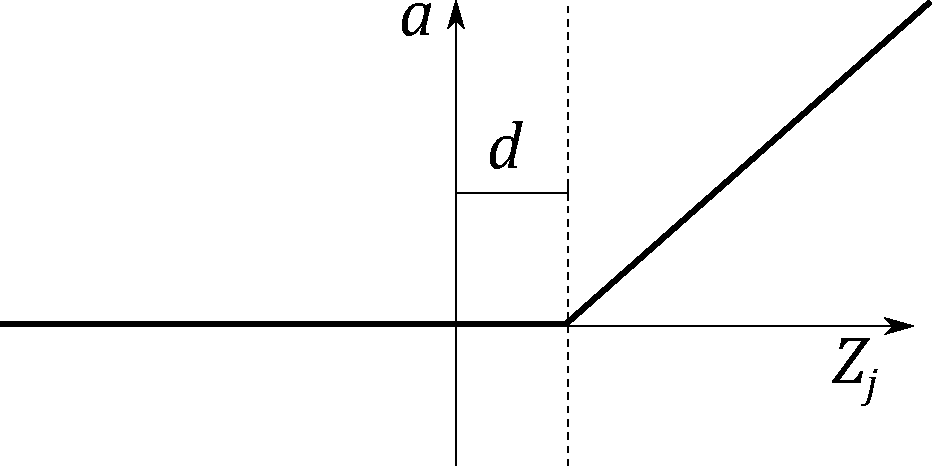
\includegraphics[width=0.5\linewidth]{images/relu.pdf}    

    \caption{In figure captions, explain what the reader is looking at: ``A schematic of the rectifying linear unit, where $a$ is the output amplitude,
    $d$ is a configurable dead-zone, and $Z_j$ is the input signal'', as well as why the reader is looking at this: 
    ``It is notable that there is no activation \emph{at all} below 0, which explains our initial results.'' 
    \textbf{Use vector image formats (.pdf) where possible}. Size figures appropriately, and do not make them over-large or too small to read.
    }

    % use the notation fig:name to cross reference a figure
    \label{fig:relu} 
\end{figure}


\begin{figure}
    \centering
    \begin{subfigure}[b]{0.45\textwidth}
        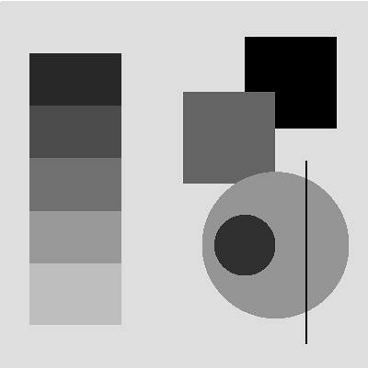
\includegraphics[width=\textwidth]{images/synthetic.png}
        \caption{Synthetic image, black on white.}
        \label{fig:syn1}
    \end{subfigure}
    ~ %add desired spacing between images, e. g. ~, \quad, \qquad, \hfill etc. 
      %(or a blank line to force the subfigure onto a new line)
    \begin{subfigure}[b]{0.45\textwidth}
        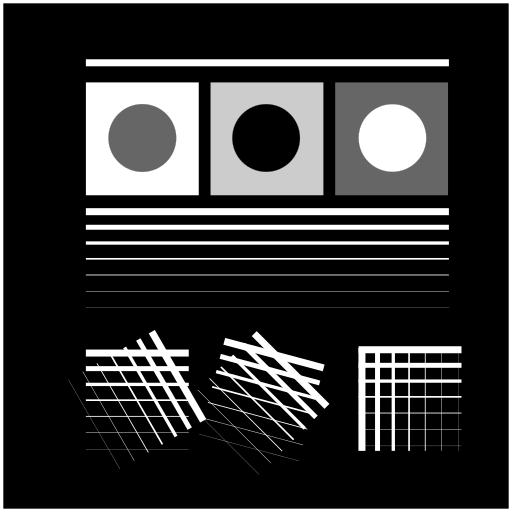
\includegraphics[width=\textwidth]{images/synthetic_2.png}
        \caption{Synthetic image, white on black.}
        \label{fig:syn2}
    \end{subfigure}
    ~ %add desired spacing between images, e. g. ~, \quad, \qquad, \hfill etc. 
    %(or a blank line to force the subfigure onto a new line)    
    \caption{Synthetic test images for edge detection algorithms. \subref{fig:syn1} shows various gray levels that require an adaptive algorithm. \subref{fig:syn2}
    shows more challenging edge detection tests that have crossing lines. Fusing these into full segments typically requires algorithms like the Hough transform.
    This is an example of using subfigures, with \texttt{subref}s in the caption.
    }\label{fig:synthetic}
\end{figure}

\clearpage

\subsection{Equations}

Equations should be typeset correctly and precisely. Make sure you get parenthesis sizing correct, and punctuate equations correctly 
(the comma is important and goes \textit{inside} the equation block). Explain any symbols used clearly if not defined earlier. 

For example, we might define:
\begin{equation}
    \hat{f}(\xi) = \frac{1}{2}\left[ \int_{-\infty}^{\infty} f(x) e^{2\pi i x \xi} \right],
\end{equation}    
where $\hat{f}(\xi)$ is the Fourier transform of the time domain signal $f(x)$.

\subsection{Algorithms}
Algorithms can be set using \texttt{algorithm2e}, as in Algorithm \ref{alg:metropolis}.

% NOTE: line ends are denoted by \; in algorithm2e
\begin{algorithm}
    \DontPrintSemicolon
    \KwData{$f_X(x)$, a probability density function returing the density at $x$.\; $\sigma$ a standard deviation specifying the spread of the proposal distribution.\;
    $x_0$, an initial starting condition.}
    \KwResult{$s=[x_1, x_2, \dots, x_n]$, $n$ samples approximately drawn from a distribution with PDF $f_X(x)$.}
    \Begin{
        $s \longleftarrow []$\;
        $p \longleftarrow f_X(x)$\;
        $i \longleftarrow 0$\;
        \While{$i < n$}
        {
            $x^\prime \longleftarrow \mathcal{N}(x, \sigma^2)$\;
            $p^\prime \longleftarrow f_X(x^\prime)$\;
            $a \longleftarrow \frac{p^\prime}{p}$\;
            $r \longleftarrow U(0,1)$\;
            \If{$r<a$}
            {
                $x \longleftarrow x^\prime$\;
                $p \longleftarrow f_X(x)$\;
                $i \longleftarrow i+1$\;
                append $x$ to $s$\;
            }
        }
    }
    
\caption{The Metropolis-Hastings MCMC algorithm for drawing samples from arbitrary probability distributions, 
specialised for normal proposal distributions $q(x^\prime|x) = \mathcal{N}(x, \sigma^2)$. The symmetry of the normal distribution means the acceptance rule takes the simplified form.}\label{alg:metropolis}
\end{algorithm}

\subsection{Tables}

If you need to include tables, like Table \ref{tab:operators}, use a tool like https://www.tablesgenerator.com/ to generate the table as it is
extremely tedious otherwise. 

\begin{table}[]
    \caption{The standard table of operators in Python, along with their functional equivalents from the \texttt{operator} package. Note that table
    captions go above the table, not below. Do not add additional rules/lines to tables. }\label{tab:operators}
    %\tt 
    \rowcolors{2}{}{gray!3}
    \begin{tabular}{@{}lll@{}}
    %\toprule
    \textbf{Operation}    & \textbf{Syntax}                & \textbf{Function}                            \\ %\midrule % optional rule for header
    Addition              & \texttt{a + b}                          & \texttt{add(a, b)}                                    \\
    Concatenation         & \texttt{seq1 + seq2}                    & \texttt{concat(seq1, seq2)}                           \\
    Containment Test      & \texttt{obj in seq}                     & \texttt{contains(seq, obj)}                           \\
    Division              & \texttt{a / b}                          & \texttt{div(a, b) }  \\
    Division              & \texttt{a / b}                          & \texttt{truediv(a, b) } \\
    Division              & \texttt{a // b}                         & \texttt{floordiv(a, b)}                               \\
    Bitwise And           & \texttt{a \& b}                         & \texttt{and\_(a, b)}                                  \\
    Bitwise Exclusive Or  & \texttt{a \textasciicircum b}           & \texttt{xor(a, b)}                                    \\
    Bitwise Inversion     & \texttt{$\sim$a}                        & \texttt{invert(a)}                                    \\
    Bitwise Or            & \texttt{a | b}                          & \texttt{or\_(a, b)}                                   \\
    Exponentiation        & \texttt{a ** b}                         & \texttt{pow(a, b)}                                    \\
    Identity              & \texttt{a is b}                         & \texttt{is\_(a, b)}                                   \\
    Identity              & \texttt{a is not b}                     & \texttt{is\_not(a, b)}                                \\
    Indexed Assignment    & \texttt{obj{[}k{]} = v}                 & \texttt{setitem(obj, k, v)}                           \\
    Indexed Deletion      & \texttt{del obj{[}k{]}}                 & \texttt{delitem(obj, k)}                              \\
    Indexing              & \texttt{obj{[}k{]}}                     & \texttt{getitem(obj, k)}                              \\
    Left Shift            & \texttt{a \textless{}\textless b}       & \texttt{lshift(a, b)}                                 \\
    Modulo                & \texttt{a \% b}                         & \texttt{mod(a, b)}                                    \\
    Multiplication        & \texttt{a * b}                          & \texttt{mul(a, b)}                                    \\
    Negation (Arithmetic) & \texttt{- a}                            & \texttt{neg(a)}                                       \\
    Negation (Logical)    & \texttt{not a}                          & \texttt{not\_(a)}                                     \\
    Positive              & \texttt{+ a}                            & \texttt{pos(a)}                                       \\
    Right Shift           & \texttt{a \textgreater{}\textgreater b} & \texttt{rshift(a, b)}                                 \\
    Sequence Repetition   & \texttt{seq * i}                        & \texttt{repeat(seq, i)}                               \\
    Slice Assignment      & \texttt{seq{[}i:j{]} = values}          & \texttt{setitem(seq, slice(i, j), values)}            \\
    Slice Deletion        & \texttt{del seq{[}i:j{]}}               & \texttt{delitem(seq, slice(i, j))}                    \\
    Slicing               & \texttt{seq{[}i:j{]}}                   & \texttt{getitem(seq, slice(i, j))}                    \\
    String Formatting     & \texttt{s \% obj}                       & \texttt{mod(s, obj)}                                  \\
    Subtraction           & \texttt{a - b}                          & \texttt{sub(a, b)}                                    \\
    Truth Test            & \texttt{obj}                            & \texttt{truth(obj)}                                   \\
    Ordering              & \texttt{a \textless b}                  & \texttt{lt(a, b)}                                     \\
    Ordering              & \texttt{a \textless{}= b}               & \texttt{le(a, b)}                                     \\
    % \bottomrule
    \end{tabular}
    \end{table}
\subsection{Code}

Avoid putting large blocks of code in the report (more than a page in one block, for example). Use syntax highlighting if possible, as in Listing \ref{lst:callahan}.

\begin{lstlisting}[language=python, float, caption={The algorithm for packing the $3\times 3$ outer-totalistic binary CA successor rule into a 
    $16\times 16\times 16\times 16$ 4 bit lookup table, running an equivalent, notionally 16-state $2\times 2$ CA.}, label=lst:callahan]
    def create_callahan_table(rule="b3s23"):
        """Generate the lookup table for the cells."""        
        s_table = np.zeros((16, 16, 16, 16), dtype=np.uint8)
        birth, survive = parse_rule(rule)

        # generate all 16 bit strings
        for iv in range(65536):
            bv = [(iv >> z) & 1 for z in range(16)]
            a, b, c, d, e, f, g, h, i, j, k, l, m, n, o, p = bv

            # compute next state of the inner 2x2
            nw = apply_rule(f, a, b, c, e, g, i, j, k)
            ne = apply_rule(g, b, c, d, f, h, j, k, l)
            sw = apply_rule(j, e, f, g, i, k, m, n, o)
            se = apply_rule(k, f, g, h, j, l, n, o, p)

            # compute the index of this 4x4
            nw_code = a | (b << 1) | (e << 2) | (f << 3)
            ne_code = c | (d << 1) | (g << 2) | (h << 3)
            sw_code = i | (j << 1) | (m << 2) | (n << 3)
            se_code = k | (l << 1) | (o << 2) | (p << 3)

            # compute the state for the 2x2
            next_code = nw | (ne << 1) | (sw << 2) | (se << 3)

            # get the 4x4 index, and write into the table
            s_table[nw_code, ne_code, sw_code, se_code] = next_code

        return s_table

\end{lstlisting}

%==================================================================================================================================
\chapter{Evaluation} 
How good is your solution? How well did you solve the general problem, and what evidence do you have to support that?

\section{Guidance}
\begin{itemize}
    \item
        Ask specific questions that address the general problem.
    \item
        Answer them with precise evidence (graphs, numbers, statistical
        analysis, qualitative analysis).
    \item
        Be fair and be scientific.
    \item
        The key thing is to show that you know how to evaluate your work, not
        that your work is the most amazing product ever.
\end{itemize}

\section{Evidence}
Make sure you present your evidence well. Use appropriate visualisations, reporting techniques and statistical analysis, as appropriate.

If you visualise, follow the basic rules, as illustrated in Figure \ref{fig:boxplot}:
\begin{itemize}
\item Label everything correctly (axis, title, units).
\item Caption thoroughly.
\item Reference in text.
\item \textbf{Include appropriate display of uncertainty (e.g. error bars, Box plot)}
\item Minimize clutter.
\end{itemize}

See the file \texttt{guide\_to\_visualising.pdf} for further information and guidance.

\begin{figure}
    \centering
    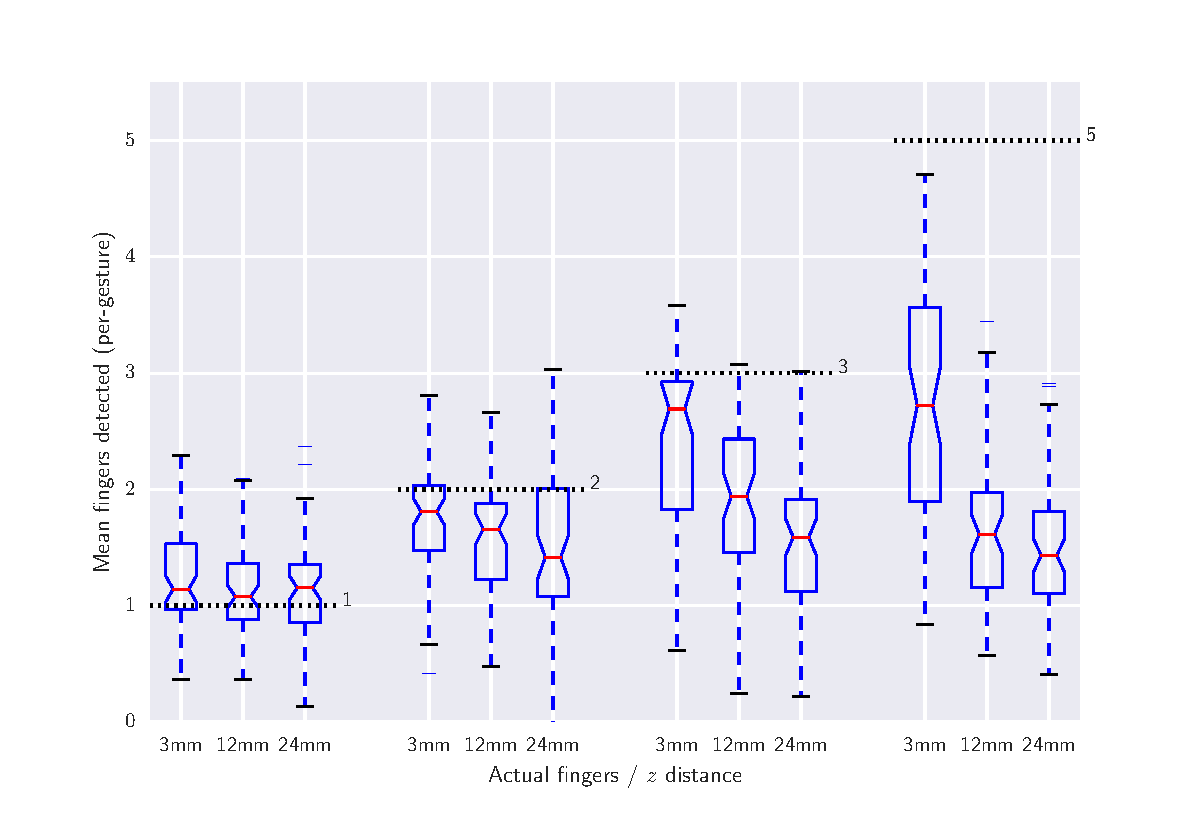
\includegraphics[width=1.0\linewidth]{images/boxplot_finger_distance.pdf}    

    \caption{Average number of fingers detected by the touch sensor at different heights above the surface, averaged over all gestures. Dashed lines indicate
    the true number of fingers present. The Box plots include bootstrapped uncertainty notches for the median. It is clear that the device is biased toward 
    undercounting fingers, particularly at higher $z$ distances.
    }

    % use the notation fig:name to cross reference a figure
    \label{fig:boxplot} 
\end{figure}


%==================================================================================================================================
\chapter{Conclusion}    
Summarise the whole project for a lazy reader who didn't read the rest (e.g. a prize-awarding committee).
\section{Guidance}
\begin{itemize}
    \item
        Summarise briefly and fairly.
    \item
        You should be addressing the general problem you introduced in the
        Introduction.        
    \item
        Include summary of concrete results (``the new compiler ran 2x
        faster'')
    \item
        Indicate what future work could be done, but remember: \textbf{you
        won't get credit for things you haven't done}.
\end{itemize}

%==================================================================================================================================
%
% 
%==================================================================================================================================
%  APPENDICES  

\begin{appendices}

\chapter{Appendices}

Typical inclusions in the appendices are:

\begin{itemize}
\item
  Copies of ethics approvals (required if obtained)
\item
  Copies of questionnaires etc. used to gather data from subjects.
\item
  Extensive tables or figures that are too bulky to fit in the main body of
  the report, particularly ones that are repetitive and summarised in the body.

\item Outline of the source code (e.g. directory structure), or other architecture documentation like class diagrams.

\item User manuals, and any guides to starting/running the software.

\end{itemize}

\textbf{Don't include your source code in the appendices}. It will be
submitted separately.

\end{appendices}

%==================================================================================================================================
%   BIBLIOGRAPHY   

% The bibliography style is abbrvnat
% The bibliography always appears last, after the appendices.

\bibliographystyle{abbrvnat}

\bibliography{l4proj}


\end{document}

